\begin{frame}{Current Progress}
    \begin{itemize}
        \item Cleaned up trench 1 of La Cuernavilla in RealityCapture
        \item Created initial mesh and subsampled it (90M to 5.5M)
        \item Cleaned it up in ZBrush (100,000 tris now)
    \end{itemize}    
\end{frame}

\begin{frame}{Renders}
    \begin{columns}[T] % Align columns at the top
        \begin{column}{0.5\textwidth}
            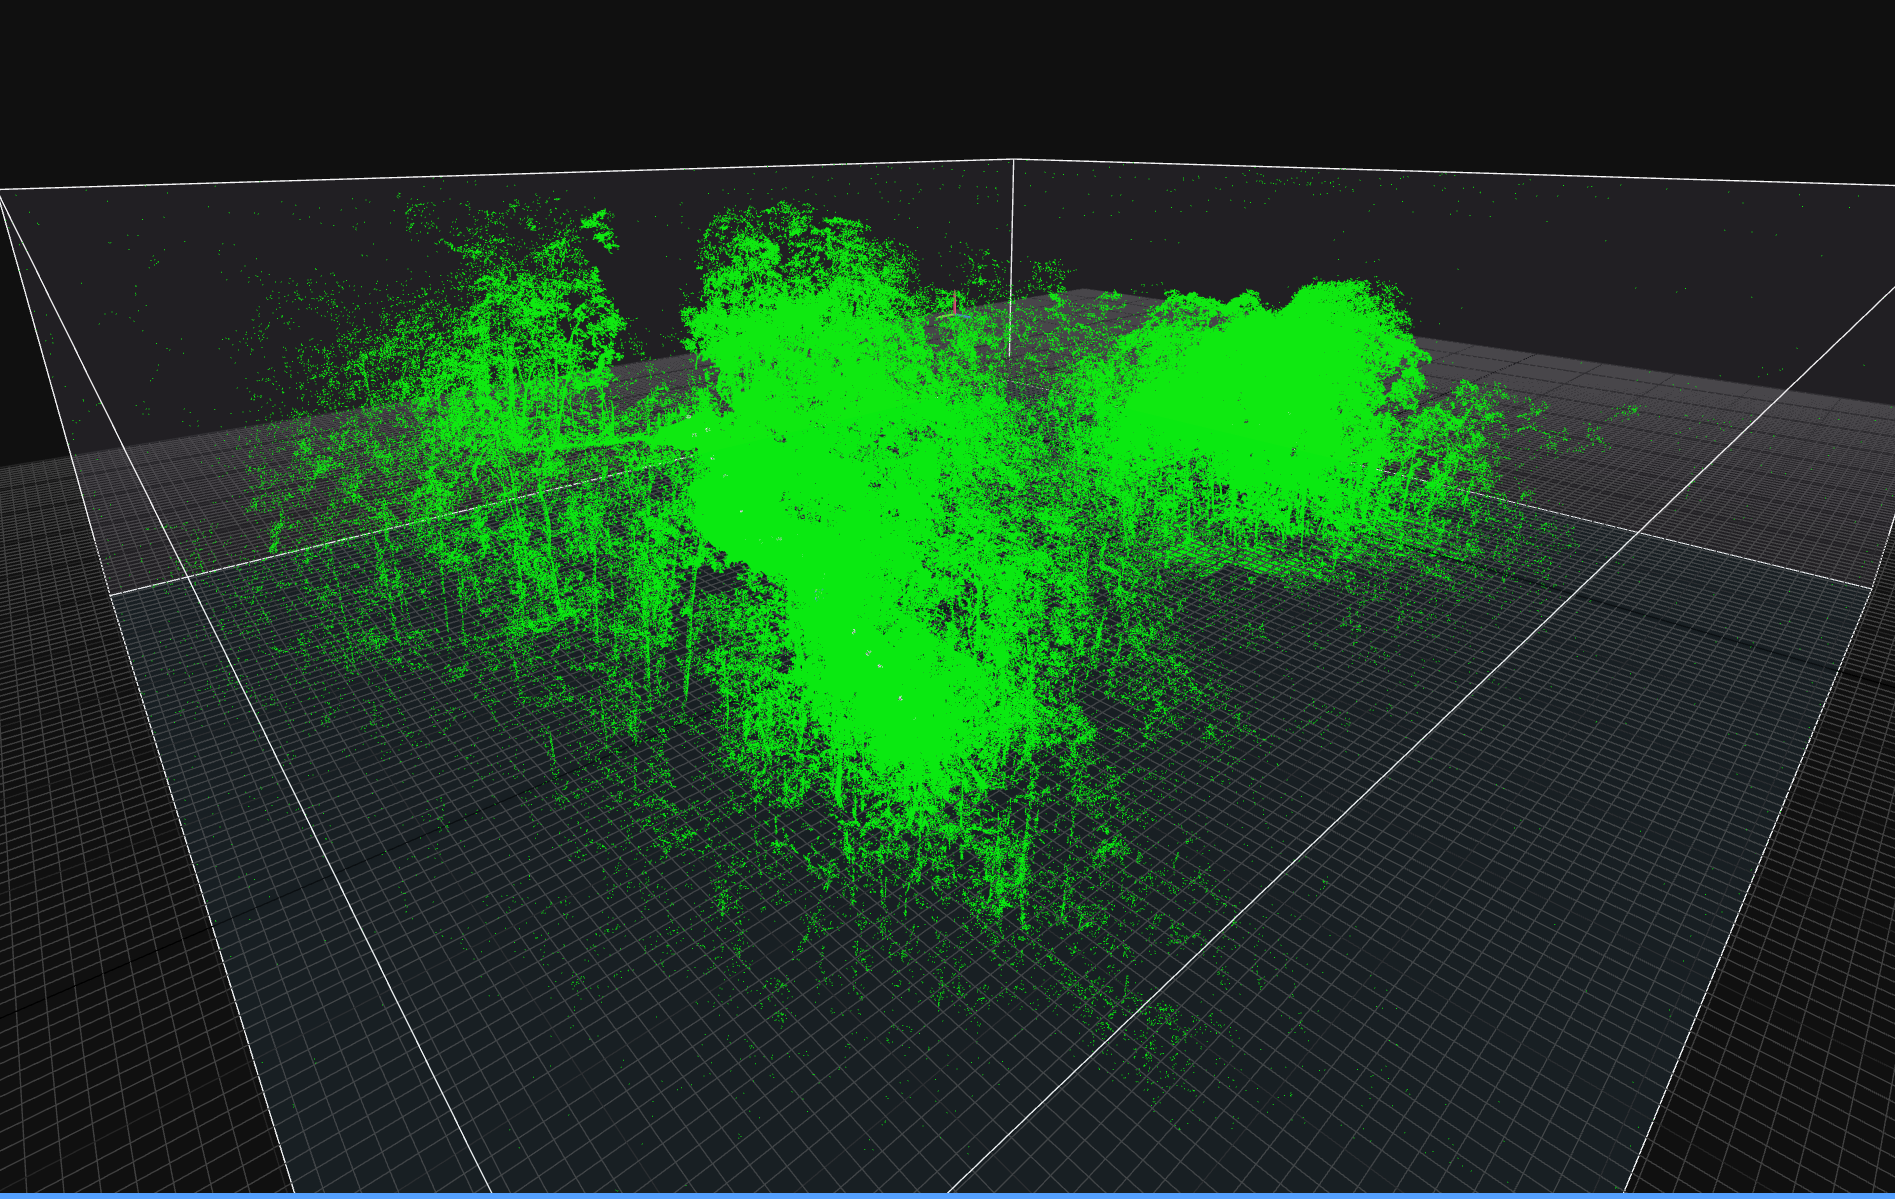
\includegraphics[width=\textwidth, keepaspectratio]{images/maya/image1.png}
        \end{column}
        \begin{column}{0.5\textwidth}
            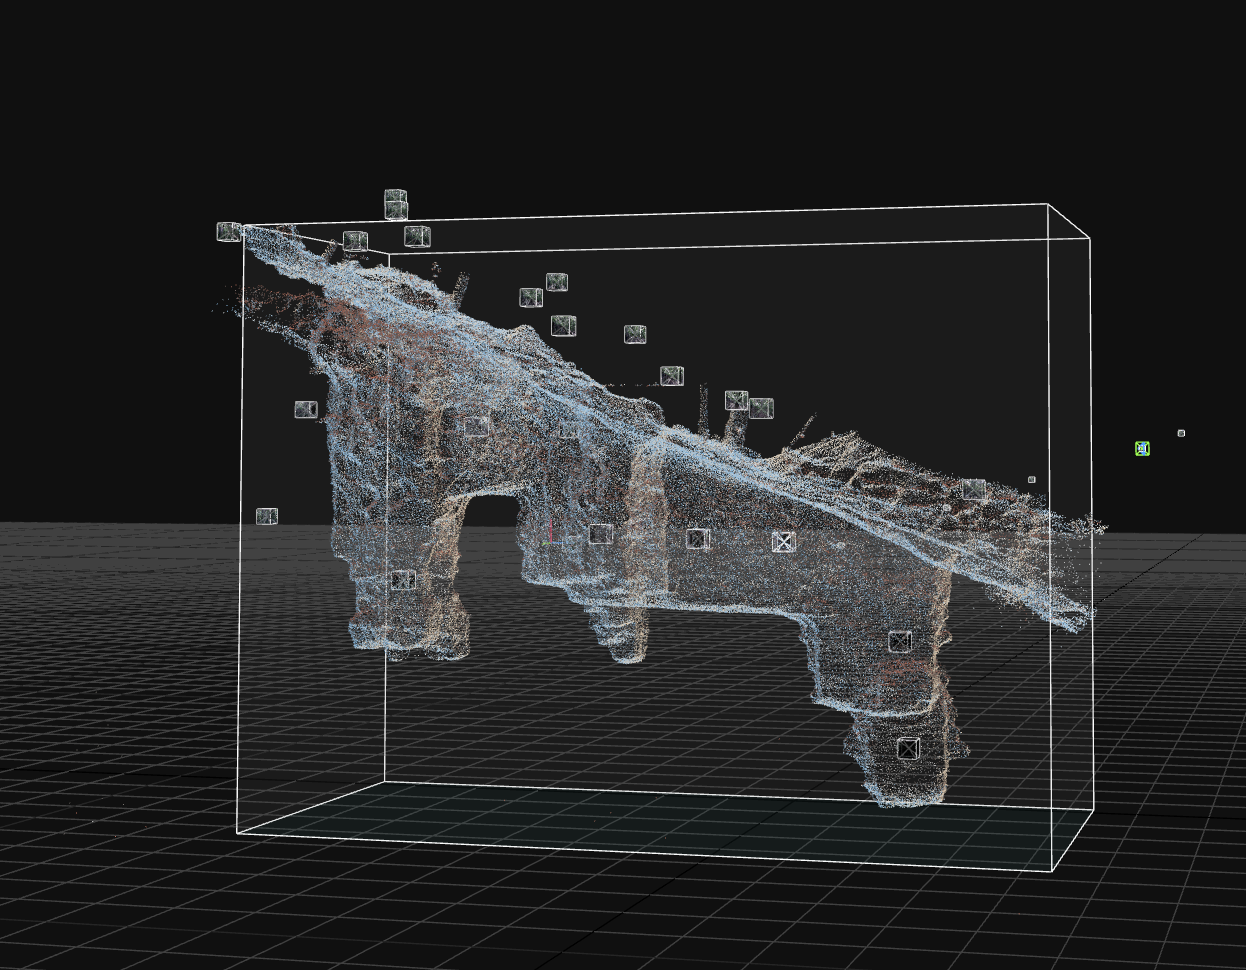
\includegraphics[width=\textwidth, keepaspectratio]{images/maya/image2.png}
        \end{column}
    \end{columns}
\end{frame}

\begin{frame}{Additional Renders}
    \begin{columns}[T] % Align columns at the top
        \begin{column}{0.5\textwidth}
            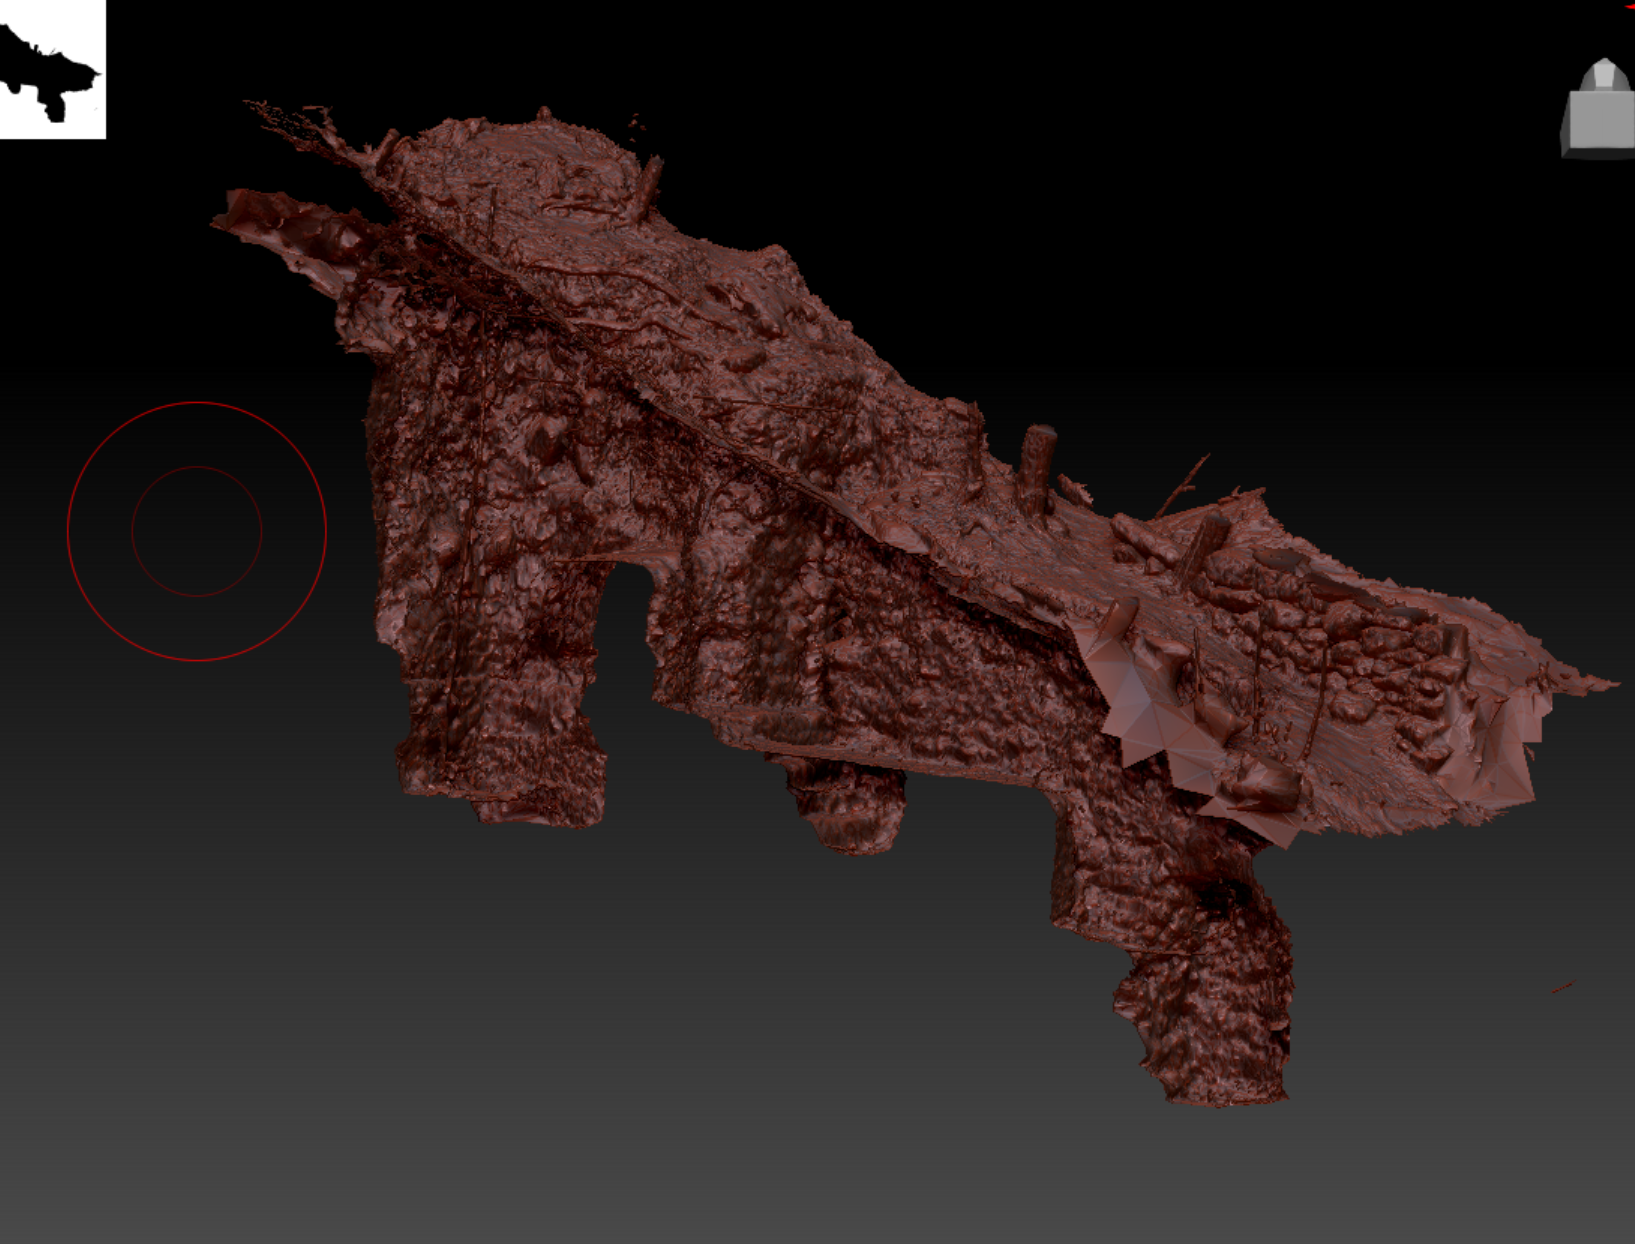
\includegraphics[width=\textwidth, keepaspectratio]{images/maya/image3.png}
        \end{column}
        \begin{column}{0.5\textwidth}
            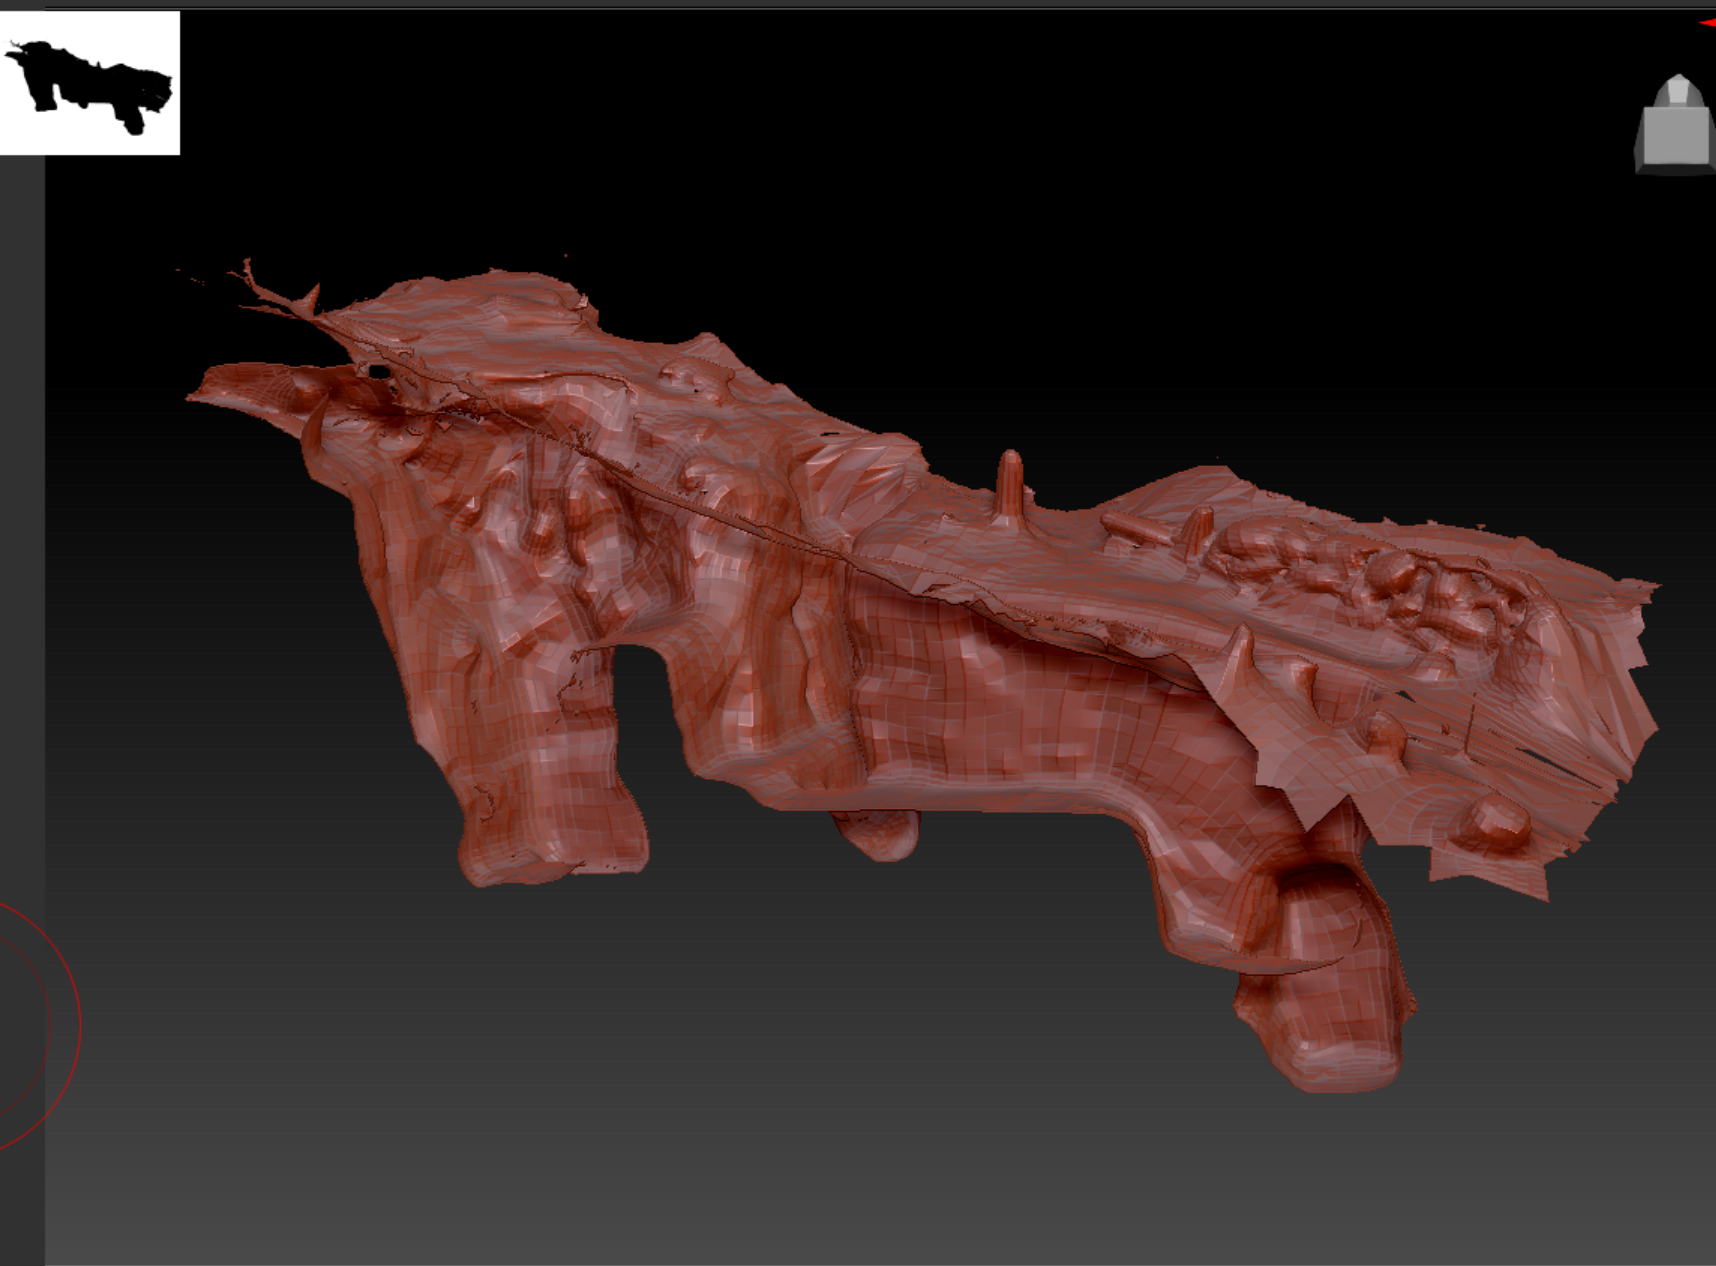
\includegraphics[width=\textwidth, keepaspectratio]{images/maya/image4.png}
        \end{column}
    \end{columns}
\end{frame}

\begin{frame}{Next Steps}
    \begin{itemize}
        \item Divide the model into smaller polygroups for easier management
        \item Retopologize
        \item Start mapping textures
        \item Subdivide the mesh to restore detail
    \end{itemize}    
\end{frame}
